\chapter{Auto-AFIDs: Automatic Anatomical Fiducial Localization} \label{chap:Autoafids}
\newpage
\sloppy
This chapter is largely based on:
\begin{itemize}[noitemsep,topsep=0pt]
	\item Taha, A., Bansal, D., Snyder, M., et al. AutoAFIDs: Automatic brain landmark detection for quality control, stereotactic targeting, and brain charting. In-Prep.
\end{itemize}

\section{Introduction}
\subsection{Brain Coordinates in Neuroimaging and Neurosurgery}
Three-dimensional Cartesian coordinates (x, y, z) offer a convenient and precise framework to represent brain structures. This abstraction underlies a broad range of applications in both neuroimaging and neurosurgical workflows, enabling reproducibility \cite{Dockes2020-nw}, cross-subject comparison \cite{Glasser2016-ko}, and multimodal data integration \cite{Uludag2014-qz}. In research, coordinates form the backbone of meta-analytic platforms such as \texttt{NeuroSynth} \cite{Yarkoni2011-sr} and \texttt{NeuroQuery} \cite{Dockes2020-nw}, which aggregate reported coordinates from thousands of studies to identify consistent associations between brain and behavior. In clinical contexts, neuromodulation targets and optimal stimulation zones are represented by coordinates relative to the major anatomical landmarks \cite{Horn2017-bi} such as anterior and posterior commissure (AC and PC), guiding trajectory planning and enabling retrospective outcome analysis. Across both domains, coordinates are a shared spatial language for modeling and navigating the brain.

\subsection{Automatic Landmark Localization}
The manual localization of brain landmarks is often time-intensive, cognitively demanding, and subject to inter-rater variability \cite{Abbass2022-lf, Lau2019-eh,Pallavaram2008-zr}. Even with detailed annotation protocols, raters require training to achieve consistency \cite{Lau2019-eh}. These challenges pose a barrier to scaling coordinate-based workflows across large datasets and neuroimaging pipelines. To address this bottleneck, deep learning (DL) methods offer a promising avenue for automatic landmark detection in brain MRI. These approaches typically fall into two paradigms: (1) coordinate regression \cite{Neupane2024-vt} and (2) heatmap-based localization \cite{Payer2016-ik}. In coordinate regression, a network directly outputs the x,y,z coordinates of each landmark (often via fully connected layers or global pooling). In heatmap-based methods, the network predicts a probability map (often a Gaussian “fuzzy” blob) for each landmark, and the peak of the heatmap is taken as the location. Heatmap regression has become especially popular because it retains spatial context and allows the network to localize landmarks in a fully convolutional manner.

\subsection{Deep Learning Approaches}
DL has revolutionized computer vision over the past decade, with regression-based convolutional networks now widely used for tasks like facial landmark detection, pose estimation, and image registration \cite{Lathuiliere2018-oy}. While medical imaging adopted these tools more gradually, fully convolutional networks—particularly U-Net and its 3D variants—have since become foundational for segmentation and anatomical localization tasks \cite{Akkus2017-eh, Falk2019-us}. Variants such as V-Net and cascaded U-Nets improve spatial precision by capturing both global context and local detail, while architectures like the spatial configuration network (SCN) \cite{Payer2016-ik, Payer2019-sn} and multi-task cascaded CNNs \cite{Zhang2017-dc} embed geometric priors to enhance performance in data-scarce settings. More recently, self-configuring pipelines like nnLandmark \cite{Ertl2025-wu} and attention-based models such as H3DE-Net \cite{Huang2025-vt} have streamlined deployment and improved model efficiency. Despite these advances, relatively limited studies have adapted such innovations to the detection of brain landmarks central to stereotactic targeting and coordinate-based neuroimaging \cite{Edwards2021-su}. Given their consistent anatomy and clinical importance, AC-PC detection represents a promising use case for applying modern deep learning techniques to improve automation, reproducibility, and standardization in brain mapping workflows.

\subsection{Limitations in the field}
Several barriers limit the broader utility of these DL techniques. First, well-annotated, publicly available datasets with standardized brain landmarks remain scarce, which constrains training, benchmarking, and validation. Second, many existing models are not open-source, are difficult to reproduce, or lack adherence to FAIR (Findable, Accessible, Interoperable, and Reusable) data principles. Third, to the best of our knowledge, no automated workflows are built in environments compatible with the Brain Imaging Data Structure (BIDS; (Gorgolewski et al., 2016)), which impedes integration with modern neuroimaging pipelines and limits accessibility for the broader scientific community. As a result, the full potential of automated coordinate-based analysis for applications such as registration quality control, brain morphometry, or lifespan brain charting remains underrealized.

\subsection{Our Proposed Approach}
In this work, we present AutoAFIDs, a BIDS-App for automatic landmark detection using deep learning. We trained and tested AutoAFIDs using a curated open-access dataset of MRI scans (n = 202) across a range of MRI field strengths (1.5, 3, and 7T) and conditions (healthy, abnormal ventricles, and neurodegenerative) with 20,000+ landmarks manually localized by human raters. AutoAFIDs demonstrated a landmark localization accuracy comparable to human raters. We showcase the broad utility of AutoAFIDs for two downstream applications which we make available to end-users: 1) quality control of image registration, 2) stereotactic target localization. By applying AutoAFIDs on over 5,000 MRI scans from individuals aged 18 to 100, we uncovered millimetric differences in brain structure that distinguish healthy brain changes from early signs of neurodegenerative disease.

\section{Methods}
\subsection{Problem Definition}
\label{sec:problemstatement}
The objective of this study is to localize anatomical fiducial points distributed across multiple brain regions using a supervised deep learning framework. Let $\mathcal{V} \subset \mathbb{R}^3$ denote a 3D brain volume, and let $\{p_1, p_2, \ldots, p_L\}$ represent the set of $L$ target landmark coordinates, where each $p_\ell \in \mathbb{R}^3$ denotes the location of the $\ell^{\text{th}}$ anatomical point of interest.

We formulate this as a regression problem in which the model learns to predict a smooth, continuous-valued distance map centered on the target landmark. For each voxel $v \in \mathcal{V}$ and landmark $\ell$, the ground truth target $D^\ell(v)$ is defined as:

\begin{equation}
D^\ell(v) = \lVert v - p_\ell \rVert_2
\end{equation}

To enhance stability and spatial resolution, we apply an exponential decay to the predicted distance map:

\begin{equation}
T^\ell(v) = \exp(-\alpha \cdot D^\ell(v))
\end{equation}

where $\alpha$ is a fixed scaling factor controlling the spatial decay rate. During training, the model is supervised to match this transformed signal using voxelwise mean squared error (MSE):

\begin{equation}
\mathcal{L} = \frac{1}{L} \sum_{\ell=1}^L \frac{1}{|\mathcal{V}|} \sum_{v \in \mathcal{V}} \left( \hat{T}^\ell(v) - T^\ell(v) \right)^2
\end{equation}

\subsection{Imaging and Coordinate Data}

We make use of landmarks defined by the Anatomical Fiducials (AFIDs) protocol, a standardized set of 32 brain landmarks manually placed on structural T1-weighted MRI scans \cite{Lau2019-eh}. These fiducials span diverse anatomical regions, including subcortical nuclei, ventricular boundaries, and midline structures such as the anterior and posterior commissures. The imaging acquisition protocols, annotation procedures, and coordinate data used here are described in detail in Chapter~\ref{chap:afidsdata} but shown in Figure \ref{fig:ch3_Figure_data} for completeness.

For model development, all curated datasets were divided into training ($n = \textbf{148}$), validation ($n = \textbf{42}$), and testing ($n = \textbf{21}$) subsets. Stratified splitting of each dataset was used to ensure representative anatomical and demographic diversity across all sets.

\begin{figure}[hbt!]
    \centering
    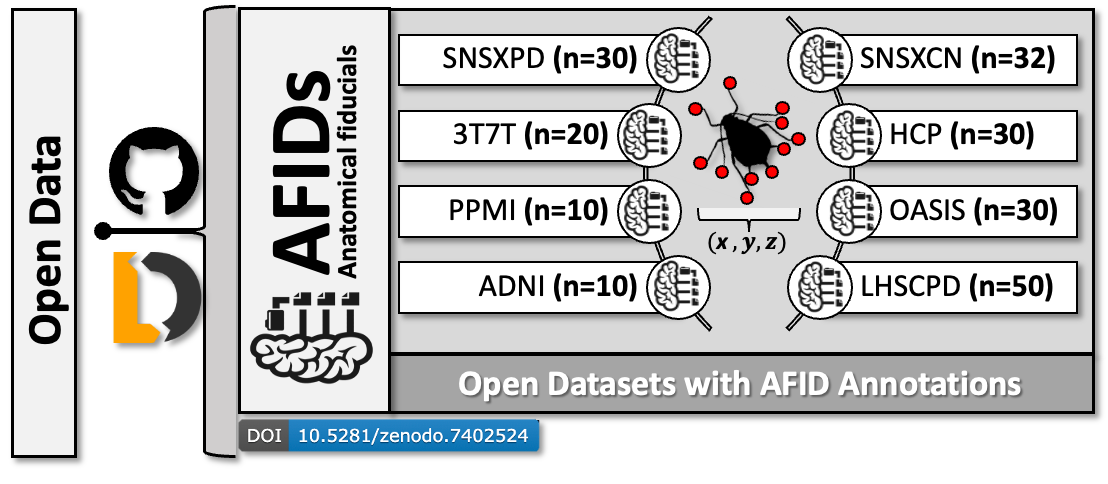
\includegraphics[width=1\linewidth]{figs/ch3_Figure_data.png}
    \caption{We make use of a previously released dataset containing anatomical fiducial (AFID) annotations. This dataset comprises eight sub-datasets spanning a range of MRI field strengths and neurodegenerative conditions. For machine learning modeling, we apply a stratified 70/20/10 split into training, validation, and test sets. By training on the combined heterogeneous dataset, the model is encouraged to learn features that are agnostic to imaging resolution, field strength, and MRI acquisition parameter differences.}
    \label{fig:ch3_Figure_data}
\end{figure}

\subsection{Preprocessing and Data Preparation}

We adopt standardized preprocessing profiles inspired by the nnU-Net framework \cite{Isensee2021-ev}, with additional modifications tailored for anatomical landmark detection. We build our workflow within a BIDS-compliant Snakemake \cite{Koster2012-ok} pipeline integrating with PyBIDS \cite{Yarkoni2019-lu} (i.e., SnakeBIDS; \url{https://github.com/khanlab/snakebids}). Input data were T1-weighted (T1w) structural MRIs, optionally converted from alternate contrasts (e.g., T2w, FLAIR, CT) using SynthSR \cite{Iglesias2023-co} when specified. 

\begin{figure}[hbt!]
    \centering
    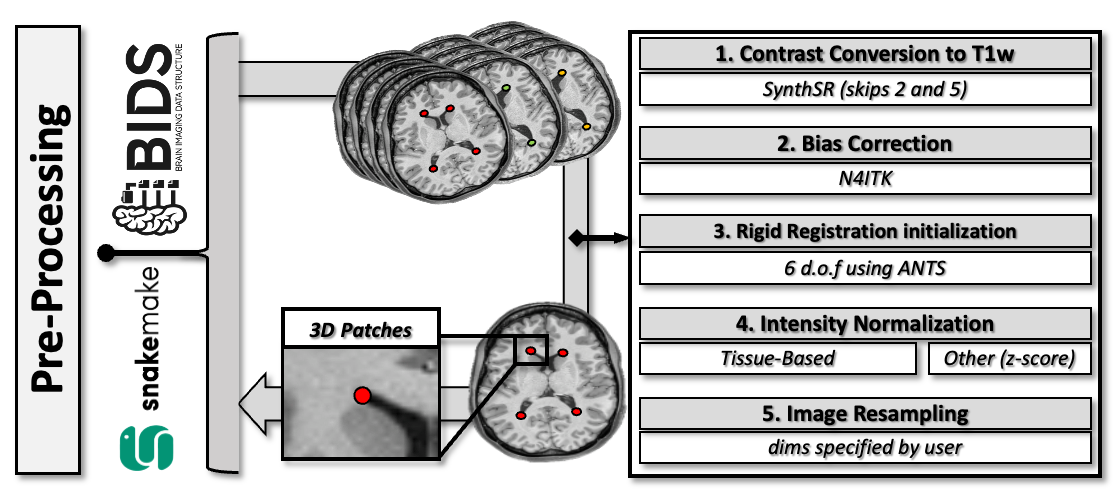
\includegraphics[width=1\linewidth]{figs/ch3_Figure_proc.png}
    \caption{Overall preprocessing pipeline employed in AutoAFIDs. Preprocessing is generally modality specific but centered around processing T1w MRI. We make use of (1) SynthSR \cite{Iglesias2023-co} to convert various modalities (e.g., T2w, CT, or FLAIR) to T1w image. Subsequently, a T1w image goes through the following preprocessing steps: (2) bias correction \cite{Tustison2010-qu}, (3) rigid registration of an annotated template for landmak priors, (4) MRI volume intensity normalization performed using various user-specified options and finally (5) resampling of the MRI volume to an isotropic resolution. The SynthSR model already outputs images that do not need to undergo preprocessing steps 2 and 5.}
    \label{fig:ch3_Figure_proc}
\end{figure}


All T1w MRI scans undergo the following steps:

\begin{enumerate}
    \item \textbf{Bias field correction:} N4 bias field correction \cite{Tustison2010-nw} is applied to mitigate intensity non-uniformities arising from scanner-related artifacts.
    
    \item \textbf{Intensity normalization:} Image intensities are normalized on a per-volume basis using robust z-score normalization, enhancing contrast between tissue boundaries relevant for landmark detection. However, we also provide the option of min-max normalization.
    
    \item \textbf{Isotropic resampling:} All volumes are resampled to a uniform 1~mm isotropic resolution to ensure consistent spatial scaling across subjects.
    
    \item \textbf{Template-to-native registration:} A rigid registration of the MNI1522009cAsym template to each subject’s native space is performed using ANTs \cite{Avants2011-zs}. This transformation is applied only to restrict the inference search space and guide patch sampling, without altering anatomical label coordinates.
    
    \item \textbf{Patch extraction:} Volumes are divided into 3D patches centered around the expected landmark region. This local patching strategy reduces memory demands and encourages finer localization.
    
    \item \textbf{Spatial augmentations:} During training, 3D patches are augmented via random rigid rotations. Each rotation is applied about a uniformly sampled axis with an angle drawn from a normal distribution with zero mean and standard deviation $\sigma_{\text{angle}}$ (in degrees), promoting rotational robustness.
\end{enumerate}

Ground-truth heatmaps for each landmark are generated by computing the voxel-wise Euclidean distance (ED) to the target coordinate and applying an exponential decay function as described in Section \ref{sec:problemstatement}.

\subsection{Patch-Based Inference}

Rather than processing the entire volume, the model predicts landmarks using a patch-based strategy. For each target landmark $\ell$, we extract a cubic patch of size $2r+1$ centered on a prior coordinate $p_\ell^{\text{prior}}$ obtained by registering a standard template (e.g., MNI space) to the subject’s native image. Let $\mathcal{P}_\ell$ denote the local patch centered on $p_\ell^{\text{prior}}$:

\begin{equation}
\mathcal{P}_\ell = \left\{ v \in \mathcal{V} \ \middle|\ \lVert v - p_\ell^{\text{prior}} \rVert_\infty \leq r \right\}
\end{equation}

The input to the network is a single-channel image patch, and the output is a distance map over $\mathcal{P}_\ell$. The predicted landmark $\hat{p}_\ell$ is extracted as the centroid of the thresholded exponential-transformed output:

\begin{equation}
\hat{p}_\ell = \text{centroid} \left( \left\{ v \in \mathcal{P}_\ell \ \middle|\ \exp(-\alpha \cdot \hat{D}^\ell(v)) > \tau \right\} \right)
\end{equation}

where $\tau$ is a percentile-based threshold (e.g., top 1\%) applied to suppress noisy responses and extract a coherent region.

\subsection{Model Architecture and Training}

Each landmark is predicted using a separate deep neural network trained independently. The shared architecture is a lightweight 3D U-Net implemented in TensorFlow. Training was performed using the Adam optimizer with early stopping on a validation set. The loss function is mean squared error between the predicted and target distance maps (after exponential transform), as described above.

\begin{figure}[hbt!]
    \centering
    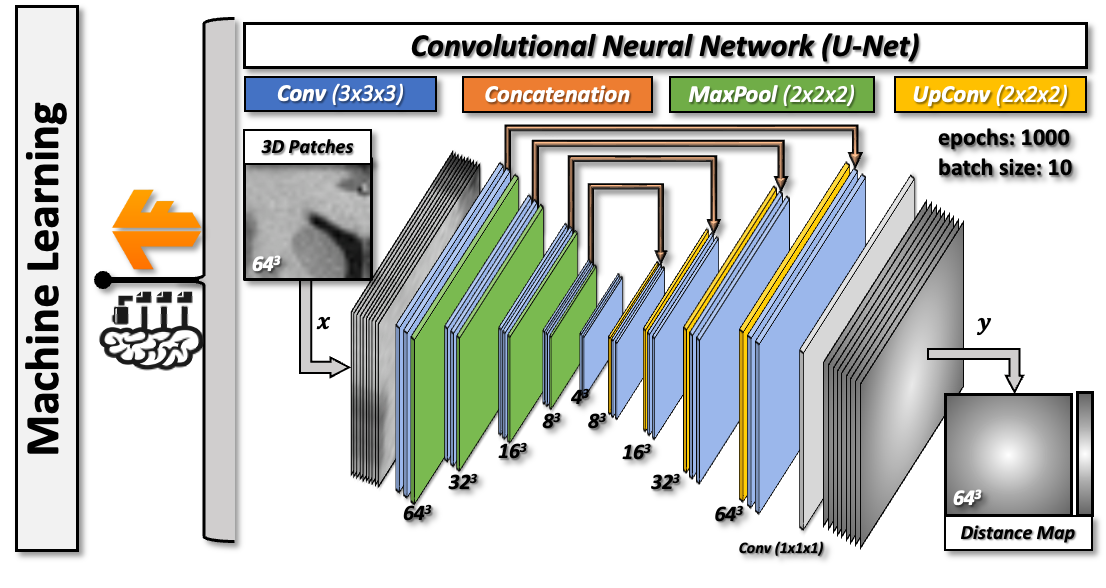
\includegraphics[width=1\linewidth]{figs/ch3_Figure_cnn.png}
    \caption{Overview of the deep learning model architecture used for anatomical fiducial localization. The model is a 3D U-Net that takes as input a 3D patch centered around a prior landmark location. The network consists of convolutional blocks (Conv, 3×3×3), downsampling via max-pooling (2×2×2), and upsampling via transposed convolutions (UpConv, 2×2×2). Skip connections concatenate encoder and decoder feature maps to preserve spatial detail. The output is a single-channel distance map representing the ED from each voxel to the target anatomical landmark.}
    \label{fig:ch3_Figure_cnn}
\end{figure}


\subsection{Model Design Rationale}
In this work, we adopt a one-network-per-landmark training strategy. While many existing approaches predict all landmarks jointly using a multi-channel output architecture, we opt for training separate models for each anatomical point. This decision is motivated by two key considerations.

First, the anatomical heterogeneity of the landmarks poses a significant modeling challenge. The AFIDs span multiple tissue types and spatial contexts—including landmarks adjacent to ventricles, embedded within white matter tracts, and lying on cortical gray matter surfaces. These diverse appearance profiles often demand different spatial priors and texture sensitivities, which a shared model may struggle to learn simultaneously. Training distinct models allows each network to specialize in the local anatomical context of its assigned landmark, without interference from competing objectives. Second, certain use cases—such as deep brain stimulation (DBS)—require sub-voxel precision in landmark localization. Errors of just a few millimeters can lead to clinically significant deviations in surgical targeting or trajectory planning. In such high-stakes applications, even minor improvements in accuracy for individual landmarks can have meaningful downstream impact. By isolating each landmark into its own dedicated model, we maximize the opportunity for hyperparameter tuning, data augmentation, and architectural adaptation tailored to each target's anatomical and clinical importance. Together, these considerations justify a modular, per-landmark approach that prioritizes accuracy and adaptability over computational efficiency.

\section{Results}
\subsection{Landmark Localization Accuracy}
Model performance was evaluated on a held-out test set (n = 21) by computing the ED between predicted and ground truth AFID coordinates. Across all 32 anatomical landmarks (672 predictions in total), the model achieved high spatial accuracy, with a median ED of 1.21 mm and an interquartile range (IQR) of 0.76–1.95 mm. Per-landmark performance showed modest variability, reflecting differences in anatomical complexity, tissue contrast, and inter-subject variability. Ten landmarks exhibited median errors in the sub-millimetric range (0.4–0.9 mm), while more challenging regions, such as those adjacent to ventricular structures, demonstrated higher variability (2-2.4 mm). The maximum observed error across all landmarks was 5.28 mm. A complete summary of per-landmark accuracy is provided in Table~\ref{tab:autoafids_accuracy}.

\subsection{Registration Evaluation Using AutoAFIDs}
To assess the utility of AutoAFIDs for evaluating registration quality, we compared its predicted landmark coordinates to those derived from Lead-DBS (v3.0; \cite{Neudorfer2023-wd}), a widely used software suite for DBS research that incorporates multi-stage nonlinear registration to align patient MRI data to MNI space. For both methods, subject-level median Euclidean distance (ED) errors were computed across all 32 AFIDs, resulting in 21 paired measurements per method. The median ED across subjects was 1.21 mm for AutoAFIDs and 1.71 mm for Lead-DBS. A Wilcoxon signed-rank test revealed a statistically significant difference in localization error (p\(<\)0.001), indicating superior performance by AutoAFIDs. The distribution of subject-level and AFID-level errors is visualized in Figure~\ref{fig:ch3_Figure_cnnvslead}a and b, respectively. AutoAFIDs statistically outperformed Lead-DBS in 14 out of 32 AFIDs. Figure~\ref{fig:ch3_Figure_cnnvslead}c shows the full distribution of all landmark EDs and their cumulative frequencies.

\begin{figure}[hbt!]
    \centering
    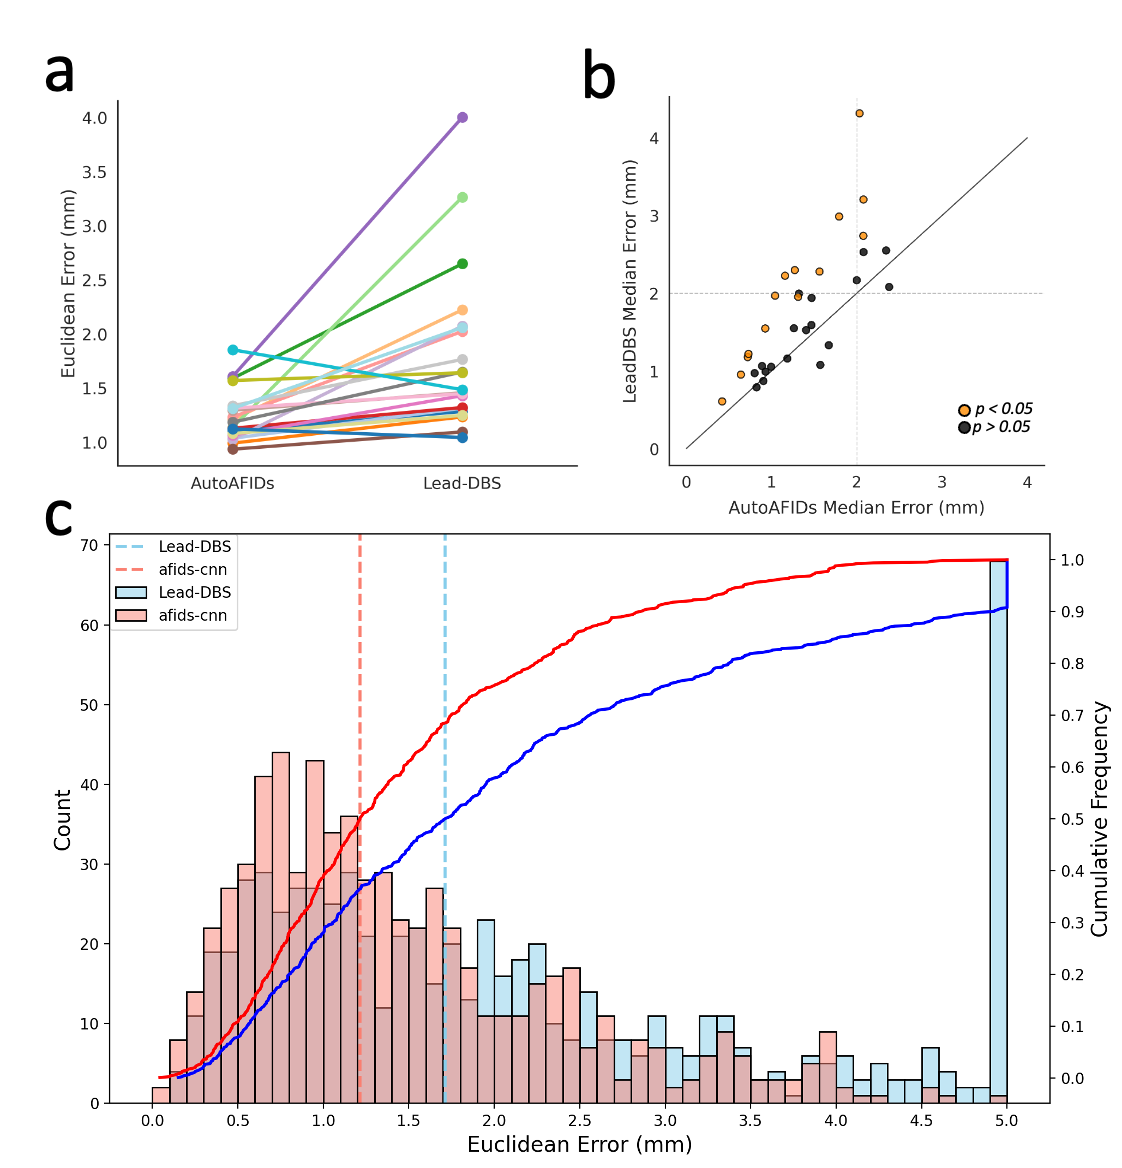
\includegraphics[width=1\linewidth]{figs/ch3_Figure_cnnvslead.png}
    \caption{Head-to-head comparison between AutoAFIDs and Lead-DBS at landmark localization in native space. (a) Subject-wise median Euclidean distance (ED) errors across all 32 landmarks. Each line connects the same subject across methods. (b) Landmark-wise comparison of median ED for AutoAFIDs versus Lead-DBS. Points are colored by Wilcoxon signed-rank test significance: orange for significant differences (p \(<\)0.05), black otherwise. Diagonal and reference lines at 2 mm are shown. (c) Distribution of all per-landmark ED values for AutoAFIDs (red) and Lead-DBS (blue), shown as overlapping histograms and cumulative frequency curves. Vertical dashed lines indicate medians.}
    \label{fig:ch3_Figure_cnnvslead}
\end{figure}

\newpage
Motivated by the variability observed in registration performance, we developed an automated QC application that uses AutoAFIDs to generate subject-specific summaries of registration accuracy. For each subject, our registration quality control tool computes descriptive statistics of ED across all 32 AFIDs. A qualitative review panel presents slice-wise visualizations for each AFID at cardinal planes with crosshairs centered on the registered and reference landmark coordinates. The report also includes a heatmap summarizing localization error by coordinate axis (x, y, z) and a 3D scatterplot visualizing landmark displacement between stereotactic space and the registered subject image. These features enable users to identify individual landmarks with high registration error, assess global alignment patterns, and quickly spot outliers. A sample report is provided in Figure~\ref{fig:figuresupregqc}.


\section{Discussion}
\section{Conclusion}



